


% This LaTeX was auto-generated from an M-file by MATLAB.
% To make changes, update the M-file and republish this document.






  
    

\section{Genetic Algorithm Tester} \label{sec:GenAlgTests}
This script file tests the function GenAlg.m program, a module in the SSA
program. The program will be tested for the relative error of the
critical factor of safety for an example slip compared to the critical
factor of safety from a paper analyzing the same example slip. Repeated
analysis of an example slip will also be performed to analyze the
consistency of the algorithm.

\subsection{Example 1}
Comparing results for the example from Greco (1996), Malkawi et al
(2001), Cheng et al (2007), Li et al (2010).

\subsubsection{Consistency Testing}
Firstly this example is used as a method of testing the consistency of
the implemented genetic algorithm. Using the same input for the genetic
algorithm to solve for the critical slip surface 15 times the physical
and critical factor of safety range the algorithm generates as critical
clip surfaces will be investigated.

For each solution a second order polynomial is fit to the vertexes
describing that solutions critical slip surface. The approximately
quadratic shape of the slip surface makes a second order polynomial an
appropriate fit. Solutions are of the form:
\[ y(x) = C_{\text{1}} \cdot x^2 + C_{\text{2}} \cdot x + C_{\text{3}} \]
Where $y$ is the vertical height of the slip surface at horizontal point
$x$. The following histograms show the spread of the fitting constants
$C_\text{1}$, $C_\text{2}$, and $C_\text{3}$. If the algorithm is
consistent the slip surfaces will follow similar shapes and the
constants will have little spread.


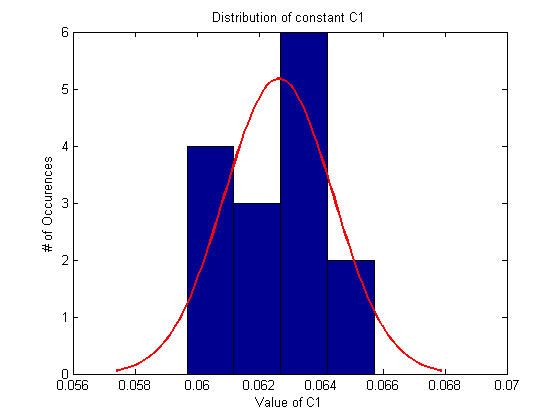
\includegraphics [width=5in]{./VV_SubDocuments/GenAlgTester_01.png}




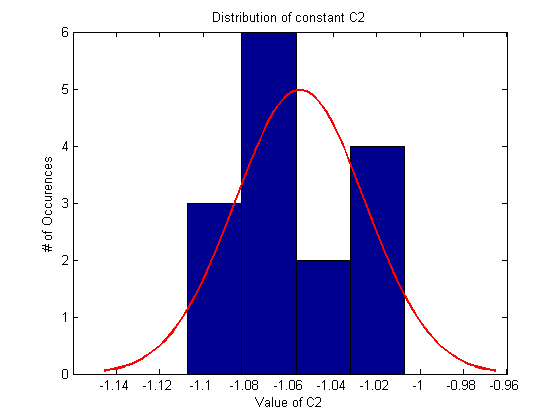
\includegraphics [width=5in]{./VV_SubDocuments/GenAlgTester_02.png}




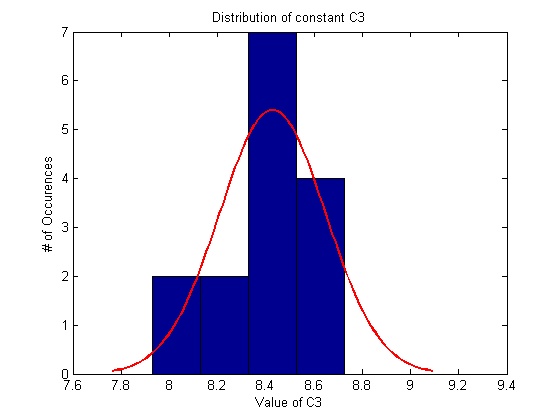
\includegraphics [width=5in]{./VV_SubDocuments/GenAlgTester_03.png}



The results in the figures show that the normal distribution of results
is approximately followed with few outlying data points, and that the
spread of the constants for the different fits is small, differing over a
small range. This suggests a consistent solution.

        
\color{lightgray} \begin{verbatim}
C1 has a standard deviation of 0.00
C2 has a standard deviation of 0.03
C3 has a standard deviation of 0.22
\end{verbatim} \color{black}
    

The next figure shows a plot of all the critical slip surfaces generated,
supporting the previous findings by showing all the slip surfaces
existing along a narrow band. The band width was measured at the entry
and exit points of the slope for context.

        
\color{lightgray} \begin{verbatim}
The entry band width was : 0.837
The exit band width was : 1.692

\end{verbatim} \color{black}
    


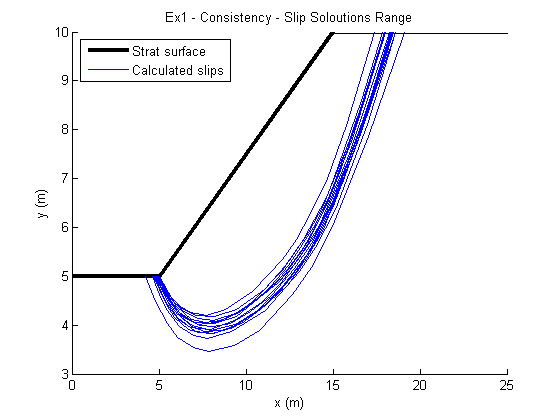
\includegraphics [width=5in]{./VV_SubDocuments/GenAlgTester_04.png}



The previous results demonstrate that the algorithm generates spatially
consistent solutions. The consistency of the Factor of Safety for the
critical slips surface will now be investigated.  The following histogram
summarizes the distribution of calculated critical factors of safety. The
figure shows a consistent factor of safety calculation, with results
differing over a small range.

        
\color{lightgray} \begin{verbatim}
The average critical slip Factor of Safety 
 is FS=1.3157, with a standard deviation 
 of 0.0036, and a minimum of FS=1.3124
\end{verbatim} \color{black}
    


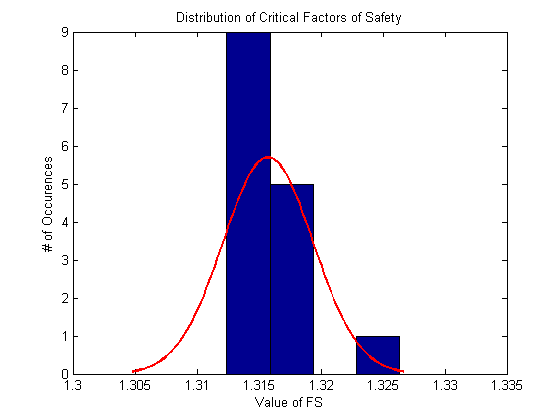
\includegraphics [width=5in]{./VV_SubDocuments/GenAlgTester_05.png}



The following figure shows the progression of the critical slip factor of
safety over each generation of the genetic algorithm. The red dot
represents the final generation. The figure generally shows convergence
after approximately 130 generations. All solutions also seem to follow
the same general path to convergence.

        
\color{lightgray} \begin{verbatim}
The average number of generations for convergence is 134
 The maximum is 319, and the minimum is 102
 The standard deviation of all trials is 55
\end{verbatim} \color{black}
    


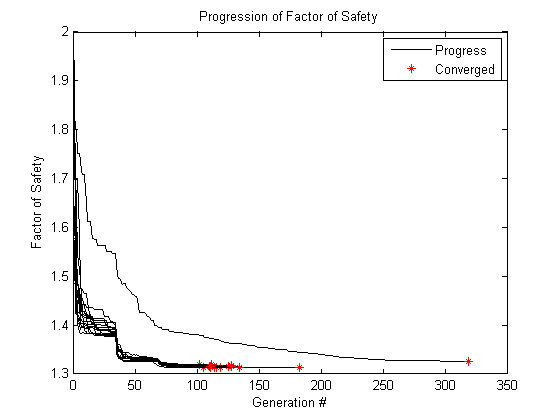
\includegraphics [width=5in]{./VV_SubDocuments/GenAlgTester_06.png}



The results seen in this section all suggest that the genetic algorithm
can consistently converge to a common critical slip, with a common
critical factor of safety.

\subsubsection{Error Test}
The Example 1 slope problem will now be measured for accuracy based on
the difference between results generated by the algorithm, and results
found scientific papers that analyzed the same example slope. A
comparison between the slip surfaces and factors of safety is made. For
this example the average of all generated slip surfaces was used.
\newline\newline\noindent
The accuracy of the slip is shown visually with a plot, and also
measured using a \textit{distance error} metric. The metric slices the
calculated slip surface, and comparison slip surface equally into 10
description vertexes. The average of distance between vertexes of the
same indice, is then considered the \textit{distance error}.
\newline\newline\noindent
The accuracy of the factor of safety is measured based on relative error
with the comparison factor of safety.

        
\color{lightgray} \begin{verbatim}
Example 1 - Slip
Author                    entry x       exit x    distance error
Calculated                 4.8225      18.2362
Greco (1996)               4.8077      18.2911          2.3715
Malkawi et al (2001)       3.5400      20.1419         10.0779
Cheng et al (2007)         4.5258      18.3943          2.9385
Li et al (2010)            4.6000      18.5300          2.7468

Example 1 - Factor of Safety
Author                         Fs     err (%)      time
Calculated                 1.3157               18.9853
Greco (1996)               1.3270      0.8494
Malkawi et al (2001)       1.2380      6.2786
Cheng et al (2007)         1.3250      0.6997
Li et al (2010)            1.3270      0.8494
\end{verbatim} \color{black}
    


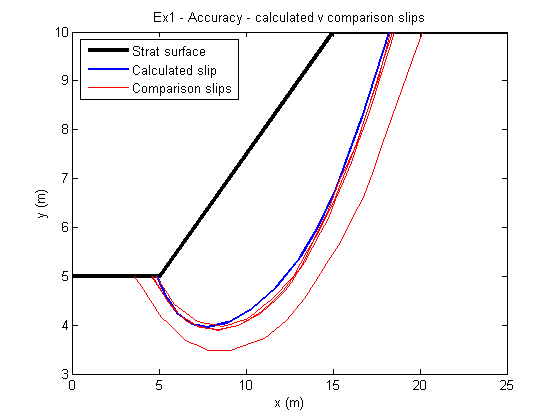
\includegraphics [width=5in]{./VV_SubDocuments/GenAlgTester_07.png}



\subsection{Examples 2-7}
Examples 2-7 compare critical factor of safety results for the program to
the results of many different papers. The tables show that results are
very accurate compared to the results in the paper, with a relative
factor of safety errors generally less than 5\% for at least one of the
comparison slips. The plots of the slip surfaces also show a critical
slip that is reasonably similar to the comparison slips.
\newline\newline\noindent
The only exception comes in Example 6. Approximately half the time a
critical factor of safety equal to the result in the paper will be
calculated, while the other half a factor of safety of approximately 0.6
will be calculated. Further investigation of this is found in
\ref{sec:Ex6Tests}.

\subsubsection*{Example 2}
\textbf{Papers:} Zolfaghari et al (2005), Cheng et al (2007),
Li et al (2010)

        
\color{lightgray} \begin{verbatim}
Example 2 - Slip
Author                    entry x       exit x    distance error
Calculated                12.6982      30.5063
Zolfaghari et al (2005)   13.0126      30.6803          0.1271
Cheng et al (2007)        12.2707      31.0044          0.1077
Li et al (2010)           12.6800      30.5300          0.0091

Example 2 - Factor of Safety
Author                         Fs     err (%)      time
Calculated                 1.1095               16.5205
Zolfaghari et al (2005)    1.2400     10.5203
Cheng et al (2007)         1.1010      0.7765
Li et al (2010)            1.1130      0.3101
\end{verbatim} \color{black}
    


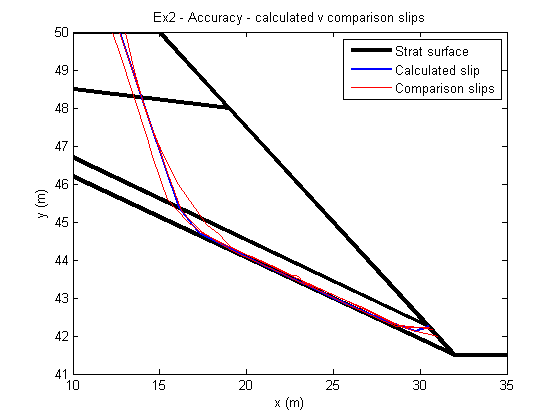
\includegraphics [width=5in]{./VV_SubDocuments/GenAlgTester_08.png}



\subsubsection*{Example 3}
\textbf{Papers:} Zolfaghari et al (2005), Cheng et al (2007),
Li et al (2010)

        
\color{lightgray} \begin{verbatim}
Example 3 - Slip
Author                    entry x       exit x    distance error
Calculated                12.5196      26.6608
Zolfaghari et al (2005)   14.4928      26.2681          0.3857
Cheng et al (2007)        12.0100      26.9014          0.1146
Li et al (2010)           12.5800      26.9200          0.0672

Example 3 - Factor of Safety
Author                         Fs     err (%)      time
Calculated                 1.3334               26.4734
Zolfaghari et al (2005)    1.4800      9.9039
Cheng et al (2007)         1.3490      1.1548
Li et al (2010)            1.3350      0.1182
\end{verbatim} \color{black}
    


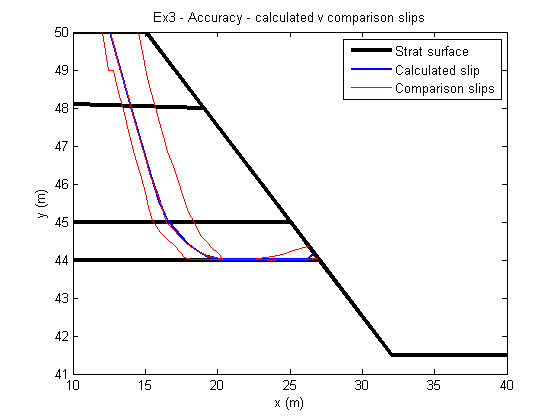
\includegraphics [width=5in]{./VV_SubDocuments/GenAlgTester_09.png}



\subsubsection*{Example 4}
\textbf{Papers:} Cheng et al (2007), Li et al (2010)

        
\color{lightgray} \begin{verbatim}
Example 4 - Slip
Author                    entry x       exit x    distance error
Calculated                13.2859      29.2819
Cheng et al (2007)        12.0749      31.9000          0.4879
Li et al (2010)           12.6500      31.9100          0.4900

Example 4 - Factor of Safety
Author                         Fs     err (%)      time
Calculated                 1.3275               26.8166
Cheng et al (2007)         1.1840     12.1204
Li et al (2010)            1.1970     10.9027
\end{verbatim} \color{black}
    


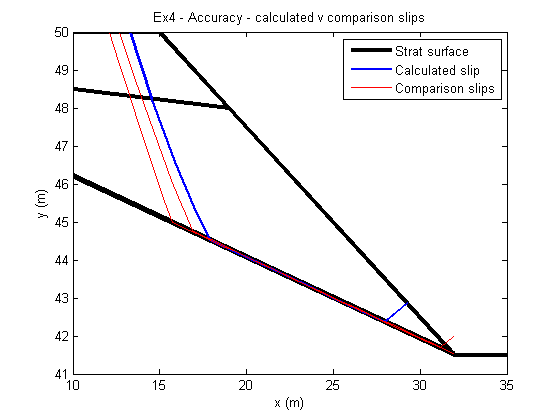
\includegraphics [width=5in]{./VV_SubDocuments/GenAlgTester_10.png}



\subsubsection*{Example 5}
\textbf{Papers:} Pham and Fredlund (2003), Li et al (2010)

        
\color{lightgray} \begin{verbatim}
Example 5 - Slip
Author                    entry x       exit x    distance err
Calculated                16.1920      40.1603
Pham and Fredlund (2003)  15.9700      43.9000          1.7744
Li et al (2010)           15.4100      41.8900          0.8691

Example 5 - factor of Safety
Author                         Fs     err (%)      time
Calculated                 1.4317               19.3441
Pham and Fredlund (2003)   1.4130      1.3233
Li et al (2010)            1.4080      1.6831
\end{verbatim} \color{black}
    


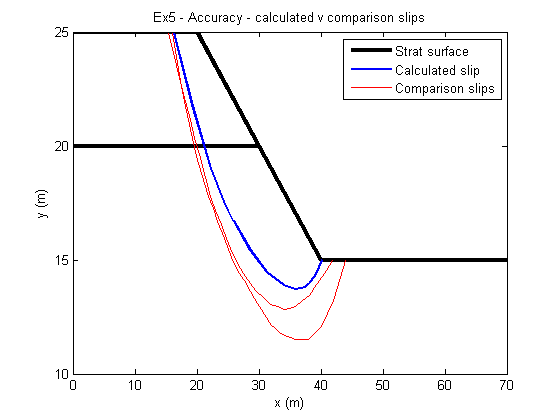
\includegraphics [width=5in]{./VV_SubDocuments/GenAlgTester_11.png}



\subsubsection*{Example 6}
\textbf{Papers:} Pham and Fredlund (2003), Li et al (2010)

        
\color{lightgray} \begin{verbatim}
Example 6 - Slip
Author                    entry x       exit x    distance error
Calculated                17.5144      44.7286
Pham and Fredlund (2003)  14.0000      47.9868          1.1717
Li et al (2010)           13.9200      49.1400          1.3511

Example 6 - Factor of Safety
Author                         Fs     err (%)      time
Calculated                 0.5215               19.0789
Pham and Fredlund (2003)   1.0000     47.8494
Li et al (2010)            1.0170     48.7212
\end{verbatim} \color{black}
    


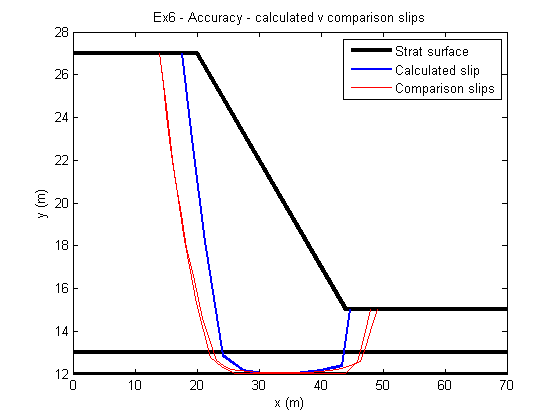
\includegraphics [width=5in]{./VV_SubDocuments/GenAlgTester_12.png}



\subsubsection*{Example 7}
\textbf{Papers:} Fredlund and Krahn (1977)

        
\color{lightgray} \begin{verbatim}
Example 7 - Slip
Author                    entry x       exit x    distance error
Calculated                12.5593      43.5584
Fredlund and Krahn (1977) 13.9714      48.3809          1.6641

Example 7 - Factor of Safety
Author                         Fs     err (%)      time
Calculated                 1.1398               18.0649
Fredlund and Krahn (1977)  1.2450      8.4466
\end{verbatim} \color{black}
    


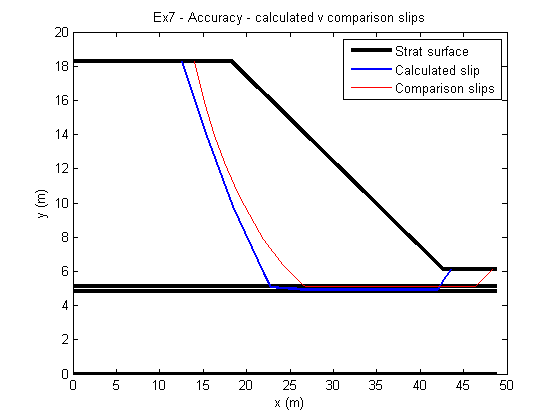
\includegraphics [width=5in]{./VV_SubDocuments/GenAlgTester_13.png}


